% Options for packages loaded elsewhere
\PassOptionsToPackage{unicode}{hyperref}
\PassOptionsToPackage{hyphens}{url}
%
\documentclass[
]{article}
\usepackage{amsmath,amssymb}
\usepackage{lmodern}
\usepackage{iftex}
\ifPDFTeX
  \usepackage[T1]{fontenc}
  \usepackage[utf8]{inputenc}
  \usepackage{textcomp} % provide euro and other symbols
\else % if luatex or xetex
  \usepackage{unicode-math}
  \defaultfontfeatures{Scale=MatchLowercase}
  \defaultfontfeatures[\rmfamily]{Ligatures=TeX,Scale=1}
\fi
% Use upquote if available, for straight quotes in verbatim environments
\IfFileExists{upquote.sty}{\usepackage{upquote}}{}
\IfFileExists{microtype.sty}{% use microtype if available
  \usepackage[]{microtype}
  \UseMicrotypeSet[protrusion]{basicmath} % disable protrusion for tt fonts
}{}
\makeatletter
\@ifundefined{KOMAClassName}{% if non-KOMA class
  \IfFileExists{parskip.sty}{%
    \usepackage{parskip}
  }{% else
    \setlength{\parindent}{0pt}
    \setlength{\parskip}{6pt plus 2pt minus 1pt}}
}{% if KOMA class
  \KOMAoptions{parskip=half}}
\makeatother
\usepackage{xcolor}
\usepackage[margin=1in]{geometry}
\usepackage{color}
\usepackage{fancyvrb}
\newcommand{\VerbBar}{|}
\newcommand{\VERB}{\Verb[commandchars=\\\{\}]}
\DefineVerbatimEnvironment{Highlighting}{Verbatim}{commandchars=\\\{\}}
% Add ',fontsize=\small' for more characters per line
\usepackage{framed}
\definecolor{shadecolor}{RGB}{248,248,248}
\newenvironment{Shaded}{\begin{snugshade}}{\end{snugshade}}
\newcommand{\AlertTok}[1]{\textcolor[rgb]{0.94,0.16,0.16}{#1}}
\newcommand{\AnnotationTok}[1]{\textcolor[rgb]{0.56,0.35,0.01}{\textbf{\textit{#1}}}}
\newcommand{\AttributeTok}[1]{\textcolor[rgb]{0.77,0.63,0.00}{#1}}
\newcommand{\BaseNTok}[1]{\textcolor[rgb]{0.00,0.00,0.81}{#1}}
\newcommand{\BuiltInTok}[1]{#1}
\newcommand{\CharTok}[1]{\textcolor[rgb]{0.31,0.60,0.02}{#1}}
\newcommand{\CommentTok}[1]{\textcolor[rgb]{0.56,0.35,0.01}{\textit{#1}}}
\newcommand{\CommentVarTok}[1]{\textcolor[rgb]{0.56,0.35,0.01}{\textbf{\textit{#1}}}}
\newcommand{\ConstantTok}[1]{\textcolor[rgb]{0.00,0.00,0.00}{#1}}
\newcommand{\ControlFlowTok}[1]{\textcolor[rgb]{0.13,0.29,0.53}{\textbf{#1}}}
\newcommand{\DataTypeTok}[1]{\textcolor[rgb]{0.13,0.29,0.53}{#1}}
\newcommand{\DecValTok}[1]{\textcolor[rgb]{0.00,0.00,0.81}{#1}}
\newcommand{\DocumentationTok}[1]{\textcolor[rgb]{0.56,0.35,0.01}{\textbf{\textit{#1}}}}
\newcommand{\ErrorTok}[1]{\textcolor[rgb]{0.64,0.00,0.00}{\textbf{#1}}}
\newcommand{\ExtensionTok}[1]{#1}
\newcommand{\FloatTok}[1]{\textcolor[rgb]{0.00,0.00,0.81}{#1}}
\newcommand{\FunctionTok}[1]{\textcolor[rgb]{0.00,0.00,0.00}{#1}}
\newcommand{\ImportTok}[1]{#1}
\newcommand{\InformationTok}[1]{\textcolor[rgb]{0.56,0.35,0.01}{\textbf{\textit{#1}}}}
\newcommand{\KeywordTok}[1]{\textcolor[rgb]{0.13,0.29,0.53}{\textbf{#1}}}
\newcommand{\NormalTok}[1]{#1}
\newcommand{\OperatorTok}[1]{\textcolor[rgb]{0.81,0.36,0.00}{\textbf{#1}}}
\newcommand{\OtherTok}[1]{\textcolor[rgb]{0.56,0.35,0.01}{#1}}
\newcommand{\PreprocessorTok}[1]{\textcolor[rgb]{0.56,0.35,0.01}{\textit{#1}}}
\newcommand{\RegionMarkerTok}[1]{#1}
\newcommand{\SpecialCharTok}[1]{\textcolor[rgb]{0.00,0.00,0.00}{#1}}
\newcommand{\SpecialStringTok}[1]{\textcolor[rgb]{0.31,0.60,0.02}{#1}}
\newcommand{\StringTok}[1]{\textcolor[rgb]{0.31,0.60,0.02}{#1}}
\newcommand{\VariableTok}[1]{\textcolor[rgb]{0.00,0.00,0.00}{#1}}
\newcommand{\VerbatimStringTok}[1]{\textcolor[rgb]{0.31,0.60,0.02}{#1}}
\newcommand{\WarningTok}[1]{\textcolor[rgb]{0.56,0.35,0.01}{\textbf{\textit{#1}}}}
\usepackage{graphicx}
\makeatletter
\def\maxwidth{\ifdim\Gin@nat@width>\linewidth\linewidth\else\Gin@nat@width\fi}
\def\maxheight{\ifdim\Gin@nat@height>\textheight\textheight\else\Gin@nat@height\fi}
\makeatother
% Scale images if necessary, so that they will not overflow the page
% margins by default, and it is still possible to overwrite the defaults
% using explicit options in \includegraphics[width, height, ...]{}
\setkeys{Gin}{width=\maxwidth,height=\maxheight,keepaspectratio}
% Set default figure placement to htbp
\makeatletter
\def\fps@figure{htbp}
\makeatother
\setlength{\emergencystretch}{3em} % prevent overfull lines
\providecommand{\tightlist}{%
  \setlength{\itemsep}{0pt}\setlength{\parskip}{0pt}}
\setcounter{secnumdepth}{-\maxdimen} % remove section numbering
\usepackage{booktabs}
\usepackage{caption}
\usepackage{longtable}
\ifLuaTeX
  \usepackage{selnolig}  % disable illegal ligatures
\fi
\IfFileExists{bookmark.sty}{\usepackage{bookmark}}{\usepackage{hyperref}}
\IfFileExists{xurl.sty}{\usepackage{xurl}}{} % add URL line breaks if available
\urlstyle{same} % disable monospaced font for URLs
\hypersetup{
  pdftitle={Grammar of Tables},
  hidelinks,
  pdfcreator={LaTeX via pandoc}}

\title{Grammar of Tables}
\author{}
\date{\vspace{-2.5em}2023-09-10}

\begin{document}
\maketitle

{
\setcounter{tocdepth}{2}
\tableofcontents
}
\hypertarget{introduction}{%
\subsection{Introduction}\label{introduction}}

Very often in Epi-reports, it's quite necessary to produce tqbles that
convey the information in the most efficiecnt way. In this lesson we
will do that using R and the grammar of tables package.

\hypertarget{learning-objectives}{%
\subsection{Learning objectives}\label{learning-objectives}}

\begin{itemize}
\item
  Use gt() to create simple table

  \begin{itemize}
  \item
    Title and subtitle
  \item
    Format percentages and round decimals
  \end{itemize}
\item
  Conditional coloring

  \begin{itemize}
  \item
    Numeric/continuous data

    \begin{itemize}
    \item
      Scale to range of values in your data (for continuous/sequential
      range)
    \item
      Discrete color scale (set numeric ranges for each color)
    \end{itemize}
  \item
    Discrete/categorical data

    \begin{itemize}
    \tightlist
    \item
      Color by text string/factor level (e.g., met, partially met, not
      met)
    \end{itemize}
  \end{itemize}
\item
  Format text by value (font color, bold,etc.)
\item
  Stratified tables (By age group or sex or both)

  \begin{itemize}
  \item
    Preparing data for stratified table
  \item
    Stub and stub head, spanner columns
  \end{itemize}
\item
  External resources for further customization

  \begin{itemize}
  \item
    Color palettes
  \item
    Borders
  \item
    kableExtra
  \end{itemize}
\end{itemize}

\hypertarget{packages-covered-in-this-lesson}{%
\subsection{Packages covered in this
lesson}\label{packages-covered-in-this-lesson}}

In this lesson, we will use the following packages:

\begin{itemize}
\item
  `gt`
\item
  \texttt{dplyr} , \texttt{tidyr} , and `purrr`.
\item
  \texttt{janitor}
\item
  \texttt{KableExtra}
\item
  \texttt{Paletteer} , \texttt{ggsci}
\end{itemize}

\hypertarget{introduction-to-the-dataset}{%
\subsection{Introduction to the
dataset}\label{introduction-to-the-dataset}}

We will use data from \textbf{Malawi HIV Program} during the four
quarters of 2019, you can access the data yourself
\href{https://dms.hiv.health.gov.mw/dataset/?tags=HIV\&res_format=XLSX\&year=2019}{here}.

First let's import the the 4 datasets at once.

\begin{verbatim}
## -- Attaching core tidyverse packages ------------------------ tidyverse 2.0.0 --
## v dplyr     1.1.3     v readr     2.1.4
## v forcats   1.0.0     v stringr   1.5.0
## v ggplot2   3.4.3     v tibble    3.2.1
## v lubridate 1.9.2     v tidyr     1.3.0
## v purrr     1.0.2     
## -- Conflicts ------------------------------------------ tidyverse_conflicts() --
## x dplyr::filter() masks stats::filter()
## x dplyr::lag()    masks stats::lag()
## i Use the conflicted package (<http://conflicted.r-lib.org/>) to force all conflicts to become errors
\end{verbatim}

Second, let's see how this data looks like :

\begin{Shaded}
\begin{Highlighting}[]
\NormalTok{data\_united }\SpecialCharTok{|\textgreater{}} 
  \FunctionTok{glimpse}\NormalTok{()}
\end{Highlighting}
\end{Shaded}

\begin{verbatim}
## Rows: 17,235
## Columns: 29
## $ region                                 <chr> "Northern Region", "Northern Re~
## $ zone                                   <chr> "Northern Zone", "Northern Zone~
## $ district                               <chr> "Chitipa", "Chitipa", "Chitipa"~
## $ traditional_authority                  <chr> "Senior TA Bulambya Songwe", "S~
## $ facility_name                          <chr> "Kapenda Health Centre", "Kapen~
## $ datim_code                             <chr> "K9u9BIAaJJT", "K9u9BIAaJJT", "~
## $ system                                 <chr> "e-mastercard", "e-mastercard",~
## $ hsector                                <chr> "Public", "Public", "Public", "~
## $ period                                 <chr> "2019 Q1", "2019 Q1", "2019 Q1"~
## $ reporting_period                       <chr> "1st month of quarter", "1st mo~
## $ sub_groups                             <chr> "All patients (checked data)", ~
## $ new_women_registered                   <dbl> 45, NA, 40, NA, 43, NA, 32, NA,~
## $ total_women_in_booking_cohort          <dbl> NA, 55, NA, 44, NA, 37, NA, 43,~
## $ not_tested_for_syphilis                <dbl> NA, 45, NA, 19, NA, 5, NA, 43, ~
## $ syphilis_negative                      <dbl> NA, 10, NA, 25, NA, 32, NA, 0, ~
## $ syphilis_positive                      <dbl> NA, 0, NA, 0, NA, 0, NA, 0, NA,~
## $ hiv_status_not_ascertained             <dbl> 4, 7, 9, 4, 9, 5, 3, 3, 4, 26, ~
## $ previous_negative                      <dbl> 0, 0, 0, 0, 0, 1, 3, 5, 1, 3, 0~
## $ previous_positive                      <dbl> 0, 0, 0, 1, 1, 0, 1, 1, 1, 3, 2~
## $ new_negative                           <dbl> 40, 47, 30, 38, 33, 31, 25, 34,~
## $ new_positive                           <dbl> 1, 1, 1, 1, 0, 0, 0, 0, 0, 0, 0~
## $ not_on_cpt                             <dbl> NA, 0, NA, 0, NA, 0, NA, 0, NA,~
## $ on_cpt                                 <dbl> NA, 1, NA, 2, NA, 0, NA, 1, NA,~
## $ no_ar_vs                               <dbl> 0, 0, 0, 0, 0, 0, 0, 0, 0, 0, 0~
## $ already_on_art_when_starting_anc       <dbl> 0, 1, 0, 1, 1, 0, 1, 1, 1, 3, 2~
## $ started_art_at_0_27_weeks_of_pregnancy <dbl> 1, 0, 1, 1, 0, 0, 0, 0, 0, 0, 0~
## $ started_art_at_28_weeks_of_preg        <dbl> 0, 0, 0, 0, 0, 0, 0, 0, 0, 0, 0~
## $ no_ar_vs_dispensed_for_infant          <dbl> NA, 0, NA, 0, NA, 0, NA, 0, NA,~
## $ ar_vs_dispensed_for_infant             <dbl> NA, 1, NA, 2, NA, 0, NA, 1, NA,~
\end{verbatim}

For the sake of convenience, we will summarize the data by quarter and
region, and keep only

\begin{Shaded}
\begin{Highlighting}[]
\NormalTok{summarized\_data }\OtherTok{\textless{}{-}}\NormalTok{ data\_united }\SpecialCharTok{|\textgreater{}} 
  \FunctionTok{group\_by}\NormalTok{(}
\NormalTok{    zone,}
\NormalTok{    period}
\NormalTok{  ) }\SpecialCharTok{|\textgreater{}} 
  \FunctionTok{summarise}\NormalTok{(}
    \FunctionTok{across}\NormalTok{(}
      \AttributeTok{.cols =} \FunctionTok{c}\NormalTok{(}
\NormalTok{        previous\_negative, }
\NormalTok{        previous\_positive, }
\NormalTok{        new\_negative, }
\NormalTok{        new\_positive,}
\NormalTok{        hiv\_status\_not\_ascertained,  }
\NormalTok{      ),}
\NormalTok{      \textbackslash{}(x) }\FunctionTok{sum}\NormalTok{(x, }\AttributeTok{na.rm =}\NormalTok{ T) }
\NormalTok{    )}
\NormalTok{  )}
\end{Highlighting}
\end{Shaded}

\begin{verbatim}
## `summarise()` has grouped output by 'zone'. You can override using the
## `.groups` argument.
\end{verbatim}

\hypertarget{creating-simple-tables}{%
\subsection{Creating simple tables}\label{creating-simple-tables}}

\hypertarget{the-grammar-and-components-of-a-table}{%
\subsubsection{The grammar and components of a
table}\label{the-grammar-and-components-of-a-table}}

`gt` is an R package that produce publication-ready table, this package
is based on an idiom called the grammar of tables that allows the user
to describe the components of any table in a consistent manner, think of
it as the ggplot2 for tables. So, in order to start using the package we
need to understand the basics of this grammar.

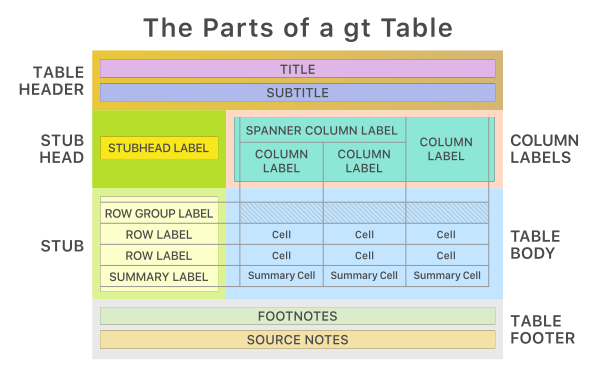
\includegraphics{images/gt_parts_of_a_table.svg}

As seen in the figure from the package website, the `gt` package
considers any table with the following components:

\begin{itemize}
\item
  he Table Header (optional; with a title and possibly a subtitle)
\item
  the Stub and the Stub Head (optional; contains row labels, optionally
  within row groups having row group labels and possibly summary labels
  when a summary is present)
\item
  the Column Labels (contains column labels, optionally under spanner
  column labels)
\item
  the Table Body (contains columns and rows of cells)
\item
  the Table Footer (optional; possibly with footnotes and source notes)
\end{itemize}

So now we will use this knowledge and combine it the syntax of the
package to actually make tables you can be proud of.

\hypertarget{a-simple-table}{%
\subsubsection{A simple table}\label{a-simple-table}}

To create a simple table from the data we got, we can simply call the
\texttt{gt()} function :

\begin{Shaded}
\begin{Highlighting}[]
\NormalTok{summarized\_data }\SpecialCharTok{|\textgreater{}} 
  \FunctionTok{gt}\NormalTok{()}
\end{Highlighting}
\end{Shaded}

\begin{longtable}{lrrrrr}
\toprule
period & previous\_negative & previous\_positive & new\_negative & new\_positive & hiv\_status\_not\_ascertained \\ 
\midrule
\multicolumn{6}{l}{Central East Zone} \\ 
\midrule
2019 Q1 & 994 & 1156 & 47471 & 616 & 2824 \\ 
2019 Q2 & 517 & 1036 & 42923 & 443 & 3209 \\ 
2019 Q3 & 1097 & 1158 & 46700 & 534 & 3583 \\ 
2019 Q4 & 595 & 1039 & 45807 & 399 & 1961 \\ 
\midrule
\multicolumn{6}{l}{Central West Zone} \\ 
\midrule
2019 Q1 & 1568 & 2526 & 75547 & 1388 & 2131 \\ 
2019 Q2 & 1322 & 2567 & 73520 & 1470 & 1804 \\ 
2019 Q3 & 1548 & 2844 & 81099 & 1382 & 1657 \\ 
2019 Q4 & 457 & 2715 & 78921 & 1292 & 1216 \\ 
\midrule
\multicolumn{6}{l}{Northern Zone} \\ 
\midrule
2019 Q1 & 675 & 1197 & 36196 & 664 & 1126 \\ 
2019 Q2 & 590 & 1084 & 35315 & 582 & 1301 \\ 
2019 Q3 & 542 & 1191 & 36850 & 570 & 954 \\ 
2019 Q4 & 346 & 1132 & 34322 & 519 & 747 \\ 
\midrule
\multicolumn{6}{l}{South East Zone} \\ 
\midrule
2019 Q1 & 1583 & 5766 & 74926 & 1976 & 1454 \\ 
2019 Q2 & 1672 & 5688 & 76937 & 1890 & 1566 \\ 
2019 Q3 & 1910 & 5966 & 80067 & 1803 & 1243 \\ 
2019 Q4 & 1504 & 5953 & 79454 & 1861 & 1385 \\ 
\midrule
\multicolumn{6}{l}{South West Zone} \\ 
\midrule
2019 Q1 & 1775 & 4171 & 50554 & 1555 & 717 \\ 
2019 Q2 & 1504 & 4726 & 53554 & 1747 & 1566 \\ 
2019 Q3 & 1394 & 4640 & 55813 & 1618 & 928 \\ 
2019 Q4 & 3391 & 4861 & 53118 & 1575 & 975 \\ 
\bottomrule
\end{longtable}

You can see already that the table is quite raw , a bit more presentable
than the output in R's console, but also two letters away compared to
what it's required to produce it in excel.

\hypertarget{adding-details-to-the-table}{%
\paragraph{Adding details to the
table}\label{adding-details-to-the-table}}

We need to add more details to the table, like a title and subtitle, we
can do that simply by using the function \texttt{tab\_heade}: and
specify the \texttt{title} and \texttt{subtitle} arguments, we can also
add the source of the data in a footnote:

\begin{Shaded}
\begin{Highlighting}[]
\NormalTok{summarized\_data }\SpecialCharTok{|\textgreater{}} 
  \FunctionTok{gt}\NormalTok{() }\SpecialCharTok{|\textgreater{}} 
  \FunctionTok{tab\_header}\NormalTok{(}
    \AttributeTok{title =} \StringTok{"Sum of cases of HIV in Malawi"}\NormalTok{,}
    \AttributeTok{subtitle =} \StringTok{"from Q1 2019 to Q2 2019"}
\NormalTok{  ) }\SpecialCharTok{|\textgreater{}} 
  \FunctionTok{tab\_source\_note}\NormalTok{(}\StringTok{"Data from the Malawi HIV Program"}\NormalTok{)}
\end{Highlighting}
\end{Shaded}

\setlength{\LTpost}{0mm}
\begin{longtable}{lrrrrr}
\caption*{
{\large Sum of cases of HIV in Malawi} \\ 
{\small from Q1 2019 to Q2 2019}
} \\ 
\toprule
period & previous\_negative & previous\_positive & new\_negative & new\_positive & hiv\_status\_not\_ascertained \\ 
\midrule
\multicolumn{6}{l}{Central East Zone} \\ 
\midrule
2019 Q1 & 994 & 1156 & 47471 & 616 & 2824 \\ 
2019 Q2 & 517 & 1036 & 42923 & 443 & 3209 \\ 
2019 Q3 & 1097 & 1158 & 46700 & 534 & 3583 \\ 
2019 Q4 & 595 & 1039 & 45807 & 399 & 1961 \\ 
\midrule
\multicolumn{6}{l}{Central West Zone} \\ 
\midrule
2019 Q1 & 1568 & 2526 & 75547 & 1388 & 2131 \\ 
2019 Q2 & 1322 & 2567 & 73520 & 1470 & 1804 \\ 
2019 Q3 & 1548 & 2844 & 81099 & 1382 & 1657 \\ 
2019 Q4 & 457 & 2715 & 78921 & 1292 & 1216 \\ 
\midrule
\multicolumn{6}{l}{Northern Zone} \\ 
\midrule
2019 Q1 & 675 & 1197 & 36196 & 664 & 1126 \\ 
2019 Q2 & 590 & 1084 & 35315 & 582 & 1301 \\ 
2019 Q3 & 542 & 1191 & 36850 & 570 & 954 \\ 
2019 Q4 & 346 & 1132 & 34322 & 519 & 747 \\ 
\midrule
\multicolumn{6}{l}{South East Zone} \\ 
\midrule
2019 Q1 & 1583 & 5766 & 74926 & 1976 & 1454 \\ 
2019 Q2 & 1672 & 5688 & 76937 & 1890 & 1566 \\ 
2019 Q3 & 1910 & 5966 & 80067 & 1803 & 1243 \\ 
2019 Q4 & 1504 & 5953 & 79454 & 1861 & 1385 \\ 
\midrule
\multicolumn{6}{l}{South West Zone} \\ 
\midrule
2019 Q1 & 1775 & 4171 & 50554 & 1555 & 717 \\ 
2019 Q2 & 1504 & 4726 & 53554 & 1747 & 1566 \\ 
2019 Q3 & 1394 & 4640 & 55813 & 1618 & 928 \\ 
2019 Q4 & 3391 & 4861 & 53118 & 1575 & 975 \\ 
\bottomrule
\end{longtable}
\begin{minipage}{\linewidth}
Data from the Malawi HIV Program\\
\end{minipage}

\hypertarget{formatting-the-values-in-the-table}{%
\paragraph{Formatting the values in the
table}\label{formatting-the-values-in-the-table}}

Great, now we know how to make a simple gt table and more details to it.
However, since we got a relatively large table with different kind of
information it can be useful to use some color scaling to add some
explanatory visual effect, say for example we want the cells with
highest values in the new\_positive column to be different from the ones
with lowest values, this, can be done in few lines of code:

\begin{Shaded}
\begin{Highlighting}[]
\NormalTok{summarized\_data }\SpecialCharTok{|\textgreater{}} 
  \FunctionTok{gt}\NormalTok{() }\SpecialCharTok{|\textgreater{}} 
  \FunctionTok{tab\_header}\NormalTok{(}
    \AttributeTok{title =} \StringTok{"Sum of cases of HIV in Malawi"}\NormalTok{,}
    \AttributeTok{subtitle =} \StringTok{"from Q1 2019 to Q2 2019"}
\NormalTok{  ) }\SpecialCharTok{|\textgreater{}} 
  \FunctionTok{tab\_source\_note}\NormalTok{(}\StringTok{"Data from the Malawi HIV Program"}\NormalTok{) }\SpecialCharTok{|\textgreater{}} 
  \FunctionTok{data\_color}\NormalTok{(}
    \AttributeTok{columns =}\NormalTok{ new\_positive,}
    \AttributeTok{fn =}\NormalTok{ scales}\SpecialCharTok{::}\FunctionTok{col\_numeric}\NormalTok{(}
      \AttributeTok{palette =} \FunctionTok{as.character}\NormalTok{(paletteer}\SpecialCharTok{::}\FunctionTok{paletteer\_d}\NormalTok{(}\StringTok{"ggsci::red\_material"}\NormalTok{, }\AttributeTok{n =} \DecValTok{10}\NormalTok{)),}
      \AttributeTok{domain =} \ConstantTok{NULL}
\NormalTok{    )}
\NormalTok{  )}
\end{Highlighting}
\end{Shaded}

\setlength{\LTpost}{0mm}
\begin{longtable}{lrrrrr}
\caption*{
{\large Sum of cases of HIV in Malawi} \\ 
{\small from Q1 2019 to Q2 2019}
} \\ 
\toprule
period & previous\_negative & previous\_positive & new\_negative & new\_positive & hiv\_status\_not\_ascertained \\ 
\midrule
\multicolumn{6}{l}{Central East Zone} \\ 
\midrule
2019 Q1 & 994 & 1156 & 47471 & 616 & 2824 \\ 
2019 Q2 & 517 & 1036 & 42923 & 443 & 3209 \\ 
2019 Q3 & 1097 & 1158 & 46700 & 534 & 3583 \\ 
2019 Q4 & 595 & 1039 & 45807 & 399 & 1961 \\ 
\midrule
\multicolumn{6}{l}{Central West Zone} \\ 
\midrule
2019 Q1 & 1568 & 2526 & 75547 & 1388 & 2131 \\ 
2019 Q2 & 1322 & 2567 & 73520 & 1470 & 1804 \\ 
2019 Q3 & 1548 & 2844 & 81099 & 1382 & 1657 \\ 
2019 Q4 & 457 & 2715 & 78921 & 1292 & 1216 \\ 
\midrule
\multicolumn{6}{l}{Northern Zone} \\ 
\midrule
2019 Q1 & 675 & 1197 & 36196 & 664 & 1126 \\ 
2019 Q2 & 590 & 1084 & 35315 & 582 & 1301 \\ 
2019 Q3 & 542 & 1191 & 36850 & 570 & 954 \\ 
2019 Q4 & 346 & 1132 & 34322 & 519 & 747 \\ 
\midrule
\multicolumn{6}{l}{South East Zone} \\ 
\midrule
2019 Q1 & 1583 & 5766 & 74926 & 1976 & 1454 \\ 
2019 Q2 & 1672 & 5688 & 76937 & 1890 & 1566 \\ 
2019 Q3 & 1910 & 5966 & 80067 & 1803 & 1243 \\ 
2019 Q4 & 1504 & 5953 & 79454 & 1861 & 1385 \\ 
\midrule
\multicolumn{6}{l}{South West Zone} \\ 
\midrule
2019 Q1 & 1775 & 4171 & 50554 & 1555 & 717 \\ 
2019 Q2 & 1504 & 4726 & 53554 & 1747 & 1566 \\ 
2019 Q3 & 1394 & 4640 & 55813 & 1618 & 928 \\ 
2019 Q4 & 3391 & 4861 & 53118 & 1575 & 975 \\ 
\bottomrule
\end{longtable}
\begin{minipage}{\linewidth}
Data from the Malawi HIV Program\\
\end{minipage}

This new function \texttt{gt::data\_color} seems a bit intimidating at
first, but the logic is straightforward:

\begin{itemize}
\item
  we specify the column we want to format it's colors in the
  \texttt{columns} argument. We can specify more than one column if the
  formatting is the same for each of them using c(\ldots).
\item
  we specify a palette of colors, the content of which should be
  characters in the hexadecimal format of color identification (eg :
  ``\#FFEBED99''). Fortunately we don't have to do this manually,
  although we could, we use the \texttt{paletteer} package to determine
  these values.
\item
  The \texttt{paletteer} package accepts value from other coloration
  packages, in our case we used \texttt{ggsci} . We defined the number
  of color shade to use(n = 10) and we passed all that to
  \texttt{as.character} to make sure that the vector of color values to
  be passed to the \texttt{data\_color} function is a vector of
  characters eventually.
\end{itemize}

We can do this for the \texttt{new\_negative} column for example, we can
use a different kind of palette, I'm using for this case the green
palette from the same package:
\href{https://github.com/nanxstats/ggsci}{\texttt{ggsci::green\_material}}
, you can find all the palettes included in the \texttt{paletteer}
package in
\href{https://emilhvitfeldt.github.io/paletteer/\#included-packages}{here}.

\begin{Shaded}
\begin{Highlighting}[]
\NormalTok{summarized\_data }\SpecialCharTok{|\textgreater{}} 
  \FunctionTok{gt}\NormalTok{() }\SpecialCharTok{|\textgreater{}} 
  \FunctionTok{tab\_header}\NormalTok{(}
    \AttributeTok{title =} \StringTok{"Sum of cases of HIV in Malawi"}\NormalTok{,}
    \AttributeTok{subtitle =} \StringTok{"from Q1 2019 to Q2 2019"}
\NormalTok{  ) }\SpecialCharTok{|\textgreater{}} 
  \FunctionTok{tab\_source\_note}\NormalTok{(}\StringTok{"Data from the Malawi HIV Program"}\NormalTok{) }\SpecialCharTok{|\textgreater{}} 
  \FunctionTok{data\_color}\NormalTok{(}
    \AttributeTok{columns =}\NormalTok{ new\_positive,}
    \AttributeTok{fn =}\NormalTok{ scales}\SpecialCharTok{::}\FunctionTok{col\_numeric}\NormalTok{(}
      \AttributeTok{palette =} \FunctionTok{as.character}\NormalTok{(paletteer}\SpecialCharTok{::}\FunctionTok{paletteer\_d}\NormalTok{(}\StringTok{"ggsci::red\_material"}\NormalTok{, }\AttributeTok{n =} \DecValTok{10}\NormalTok{)),}
      \AttributeTok{domain =} \ConstantTok{NULL}
\NormalTok{    )}
\NormalTok{  ) }\SpecialCharTok{|\textgreater{}} 
  \FunctionTok{data\_color}\NormalTok{(}
    \AttributeTok{columns =}\NormalTok{ new\_negative,}
    \AttributeTok{fn =}\NormalTok{ scales}\SpecialCharTok{::}\FunctionTok{col\_numeric}\NormalTok{(}
      \AttributeTok{palette =} \FunctionTok{as.character}\NormalTok{(paletteer}\SpecialCharTok{::}\FunctionTok{paletteer\_d}\NormalTok{(}\StringTok{"ggsci::green\_material"}\NormalTok{,}\AttributeTok{n =} \DecValTok{10}\NormalTok{)),}
      \AttributeTok{domain =} \ConstantTok{NULL}
\NormalTok{    )}
\NormalTok{  ) }
\end{Highlighting}
\end{Shaded}

\setlength{\LTpost}{0mm}
\begin{longtable}{lrrrrr}
\caption*{
{\large Sum of cases of HIV in Malawi} \\ 
{\small from Q1 2019 to Q2 2019}
} \\ 
\toprule
period & previous\_negative & previous\_positive & new\_negative & new\_positive & hiv\_status\_not\_ascertained \\ 
\midrule
\multicolumn{6}{l}{Central East Zone} \\ 
\midrule
2019 Q1 & 994 & 1156 & 47471 & 616 & 2824 \\ 
2019 Q2 & 517 & 1036 & 42923 & 443 & 3209 \\ 
2019 Q3 & 1097 & 1158 & 46700 & 534 & 3583 \\ 
2019 Q4 & 595 & 1039 & 45807 & 399 & 1961 \\ 
\midrule
\multicolumn{6}{l}{Central West Zone} \\ 
\midrule
2019 Q1 & 1568 & 2526 & 75547 & 1388 & 2131 \\ 
2019 Q2 & 1322 & 2567 & 73520 & 1470 & 1804 \\ 
2019 Q3 & 1548 & 2844 & 81099 & 1382 & 1657 \\ 
2019 Q4 & 457 & 2715 & 78921 & 1292 & 1216 \\ 
\midrule
\multicolumn{6}{l}{Northern Zone} \\ 
\midrule
2019 Q1 & 675 & 1197 & 36196 & 664 & 1126 \\ 
2019 Q2 & 590 & 1084 & 35315 & 582 & 1301 \\ 
2019 Q3 & 542 & 1191 & 36850 & 570 & 954 \\ 
2019 Q4 & 346 & 1132 & 34322 & 519 & 747 \\ 
\midrule
\multicolumn{6}{l}{South East Zone} \\ 
\midrule
2019 Q1 & 1583 & 5766 & 74926 & 1976 & 1454 \\ 
2019 Q2 & 1672 & 5688 & 76937 & 1890 & 1566 \\ 
2019 Q3 & 1910 & 5966 & 80067 & 1803 & 1243 \\ 
2019 Q4 & 1504 & 5953 & 79454 & 1861 & 1385 \\ 
\midrule
\multicolumn{6}{l}{South West Zone} \\ 
\midrule
2019 Q1 & 1775 & 4171 & 50554 & 1555 & 717 \\ 
2019 Q2 & 1504 & 4726 & 53554 & 1747 & 1566 \\ 
2019 Q3 & 1394 & 4640 & 55813 & 1618 & 928 \\ 
2019 Q4 & 3391 & 4861 & 53118 & 1575 & 975 \\ 
\bottomrule
\end{longtable}
\begin{minipage}{\linewidth}
Data from the Malawi HIV Program\\
\end{minipage}

We can also set up the table to conditionally change the color of the
text in the table depending on the value of that text. In this following
case we wanted to highlight values in the column previous positive
according to a threshold, if the value is greater than 2000 then the
text color should be red, if it's less than 2000 then the text color
should be green, we also added the styling bold to the text as well.
It's the same process, the only difference is that we specify the
condition of the formatting in the \texttt{locations} function using the
\texttt{row} argument.

\begin{Shaded}
\begin{Highlighting}[]
\NormalTok{summarized\_data }\SpecialCharTok{|\textgreater{}} 
  \FunctionTok{gt}\NormalTok{() }\SpecialCharTok{|\textgreater{}} 
  \FunctionTok{tab\_header}\NormalTok{(}
    \AttributeTok{title =} \StringTok{"Sum of cases of HIV in Malawi"}\NormalTok{,}
    \AttributeTok{subtitle =} \StringTok{"from Q1 2019 to Q2 2019"}
\NormalTok{  ) }\SpecialCharTok{|\textgreater{}} 
  \FunctionTok{tab\_source\_note}\NormalTok{(}\StringTok{"Data from the Malawi HIV Program"}\NormalTok{) }\SpecialCharTok{|\textgreater{}} 
  \FunctionTok{data\_color}\NormalTok{(}
    \AttributeTok{columns =}\NormalTok{ new\_positive,}
    \AttributeTok{fn =}\NormalTok{ scales}\SpecialCharTok{::}\FunctionTok{col\_numeric}\NormalTok{(}
      \AttributeTok{palette =} \FunctionTok{as.character}\NormalTok{(paletteer}\SpecialCharTok{::}\FunctionTok{paletteer\_d}\NormalTok{(}\StringTok{"ggsci::red\_material"}\NormalTok{, }\AttributeTok{n =} \DecValTok{10}\NormalTok{)),}
      \AttributeTok{domain =} \ConstantTok{NULL}
\NormalTok{    )}
\NormalTok{  ) }\SpecialCharTok{|\textgreater{}} 
  \FunctionTok{data\_color}\NormalTok{(}
    \AttributeTok{columns =}\NormalTok{ new\_negative,}
    \AttributeTok{fn =}\NormalTok{ scales}\SpecialCharTok{::}\FunctionTok{col\_numeric}\NormalTok{(}
      \AttributeTok{palette =} \FunctionTok{as.character}\NormalTok{(paletteer}\SpecialCharTok{::}\FunctionTok{paletteer\_d}\NormalTok{(}\StringTok{"ggsci::green\_material"}\NormalTok{,}\AttributeTok{n =} \DecValTok{10}\NormalTok{)),}
      \AttributeTok{domain =} \ConstantTok{NULL}
\NormalTok{    )}
\NormalTok{  ) }\SpecialCharTok{|\textgreater{}} 
  \FunctionTok{tab\_style}\NormalTok{(}
    \AttributeTok{style =} \FunctionTok{cell\_text}\NormalTok{(}
      \AttributeTok{color =} \StringTok{"red"}\NormalTok{,}
      \AttributeTok{weight =} \StringTok{"bold"}\NormalTok{,}
\NormalTok{    ),}
    \AttributeTok{locations =} \FunctionTok{cells\_body}\NormalTok{(}
      \AttributeTok{columns =}\NormalTok{ previous\_positive,}
      \AttributeTok{rows =}\NormalTok{ previous\_positive }\SpecialCharTok{\textgreater{}} \DecValTok{2000}
\NormalTok{    )}
\NormalTok{  )}\SpecialCharTok{|\textgreater{}} 
  \FunctionTok{tab\_style}\NormalTok{(}
    \AttributeTok{style =} \FunctionTok{cell\_text}\NormalTok{(}
      \AttributeTok{color =} \StringTok{"green"}\NormalTok{,}
      \AttributeTok{weight =} \StringTok{"bold"}\NormalTok{,}
\NormalTok{    ),}
    \AttributeTok{locations =} \FunctionTok{cells\_body}\NormalTok{(}
      \AttributeTok{columns =}\NormalTok{ previous\_positive,}
      \AttributeTok{rows =}\NormalTok{ previous\_positive }\SpecialCharTok{\textless{}} \DecValTok{2000}
\NormalTok{    )}
\NormalTok{  )}
\end{Highlighting}
\end{Shaded}

\setlength{\LTpost}{0mm}
\begin{longtable}{lrrrrr}
\caption*{
{\large Sum of cases of HIV in Malawi} \\ 
{\small from Q1 2019 to Q2 2019}
} \\ 
\toprule
period & previous\_negative & previous\_positive & new\_negative & new\_positive & hiv\_status\_not\_ascertained \\ 
\midrule
\multicolumn{6}{l}{Central East Zone} \\ 
\midrule
2019 Q1 & 994 & 1156 & 47471 & 616 & 2824 \\ 
2019 Q2 & 517 & 1036 & 42923 & 443 & 3209 \\ 
2019 Q3 & 1097 & 1158 & 46700 & 534 & 3583 \\ 
2019 Q4 & 595 & 1039 & 45807 & 399 & 1961 \\ 
\midrule
\multicolumn{6}{l}{Central West Zone} \\ 
\midrule
2019 Q1 & 1568 & 2526 & 75547 & 1388 & 2131 \\ 
2019 Q2 & 1322 & 2567 & 73520 & 1470 & 1804 \\ 
2019 Q3 & 1548 & 2844 & 81099 & 1382 & 1657 \\ 
2019 Q4 & 457 & 2715 & 78921 & 1292 & 1216 \\ 
\midrule
\multicolumn{6}{l}{Northern Zone} \\ 
\midrule
2019 Q1 & 675 & 1197 & 36196 & 664 & 1126 \\ 
2019 Q2 & 590 & 1084 & 35315 & 582 & 1301 \\ 
2019 Q3 & 542 & 1191 & 36850 & 570 & 954 \\ 
2019 Q4 & 346 & 1132 & 34322 & 519 & 747 \\ 
\midrule
\multicolumn{6}{l}{South East Zone} \\ 
\midrule
2019 Q1 & 1583 & 5766 & 74926 & 1976 & 1454 \\ 
2019 Q2 & 1672 & 5688 & 76937 & 1890 & 1566 \\ 
2019 Q3 & 1910 & 5966 & 80067 & 1803 & 1243 \\ 
2019 Q4 & 1504 & 5953 & 79454 & 1861 & 1385 \\ 
\midrule
\multicolumn{6}{l}{South West Zone} \\ 
\midrule
2019 Q1 & 1775 & 4171 & 50554 & 1555 & 717 \\ 
2019 Q2 & 1504 & 4726 & 53554 & 1747 & 1566 \\ 
2019 Q3 & 1394 & 4640 & 55813 & 1618 & 928 \\ 
2019 Q4 & 3391 & 4861 & 53118 & 1575 & 975 \\ 
\bottomrule
\end{longtable}
\begin{minipage}{\linewidth}
Data from the Malawi HIV Program\\
\end{minipage}

\hypertarget{fonts-and-text}{%
\paragraph{Fonts and text}\label{fonts-and-text}}

Now is a good time to add some customization to the text in the table.
We can do that via the function \texttt{gt::tab\_style}. We can use this
function not only to change the values in table's body, but also to any
other part of it as well.

Let's change the font and color of the title and the subtitle for
example, I'm choosing to use the \texttt{Yanone\ Kaffeesatz} font from
google. Google fonts provide you with hundreds of thousands of fonts and
styles to choose from that can be more interesting than the boring rigid
excel fonts.

In order to do that, we need to specify some details in
\texttt{gt::tab\_style} function:

\begin{itemize}
\item
  We assign a list to the argument \texttt{style}.
\item
  In that list we specify that we are editing text (i.e table specific
  values, not borders or shapes) using the function \texttt{cell\_text}.
\item
  Inside \texttt{cell\_text} we specify the details we want, i.e the
  font and the color
\item
  Finally, we add another argument to the \texttt{tab\_style} function
  that depict the location of these changes or specifications, in our
  case it's the title and the sub\_title, so we assign list to the
  \texttt{locations} argument that contains the function
  \texttt{cells\_title} which specifies the location of these changes
  we've done using the syntax below.
\item
  Note that in order to make changes to the appearance of either the
  title or subtitle, you can simple use :
  \texttt{locations\ =\ list(cells\_title(groups\ =\ "title"))} to apply
  changes to the title, or
  \texttt{locations\ =\ list(cells\_title(groups\ =\ "subtitle"))} , to
  apply changes to the subtitle without the need to use \texttt{c(…)} .
\end{itemize}

\begin{Shaded}
\begin{Highlighting}[]
\NormalTok{summarized\_data }\SpecialCharTok{|\textgreater{}} 
  \FunctionTok{gt}\NormalTok{() }\SpecialCharTok{|\textgreater{}} 
  \FunctionTok{tab\_header}\NormalTok{(}
    \AttributeTok{title =} \StringTok{"Sum of cases of HIV in Malawi"}\NormalTok{,}
    \AttributeTok{subtitle =} \StringTok{"from Q1 2019 to Q2 2019"}
\NormalTok{  ) }\SpecialCharTok{|\textgreater{}} 
  \FunctionTok{tab\_source\_note}\NormalTok{(}\StringTok{"Data from the Malawi HIV Program"}\NormalTok{) }\SpecialCharTok{|\textgreater{}} 
  \FunctionTok{data\_color}\NormalTok{(}
    \AttributeTok{columns =}\NormalTok{ new\_positive,}
    \AttributeTok{fn =}\NormalTok{ scales}\SpecialCharTok{::}\FunctionTok{col\_numeric}\NormalTok{(}
      \AttributeTok{palette =} \FunctionTok{as.character}\NormalTok{(paletteer}\SpecialCharTok{::}\FunctionTok{paletteer\_d}\NormalTok{(}\StringTok{"ggsci::red\_material"}\NormalTok{, }\AttributeTok{n =} \DecValTok{10}\NormalTok{)),}
      \AttributeTok{domain =} \ConstantTok{NULL}
\NormalTok{    )}
\NormalTok{  ) }\SpecialCharTok{|\textgreater{}} 
  \FunctionTok{data\_color}\NormalTok{(}
    \AttributeTok{columns =}\NormalTok{ new\_negative,}
    \AttributeTok{fn =}\NormalTok{ scales}\SpecialCharTok{::}\FunctionTok{col\_numeric}\NormalTok{(}
      \AttributeTok{palette =} \FunctionTok{as.character}\NormalTok{(paletteer}\SpecialCharTok{::}\FunctionTok{paletteer\_d}\NormalTok{(}\StringTok{"ggsci::green\_material"}\NormalTok{,}\AttributeTok{n =} \DecValTok{10}\NormalTok{)),}
      \AttributeTok{domain =} \ConstantTok{NULL}
\NormalTok{    )}
\NormalTok{  ) }\SpecialCharTok{|\textgreater{}} 
  \FunctionTok{tab\_style}\NormalTok{(}
    \AttributeTok{style =} \FunctionTok{cell\_text}\NormalTok{(}
      \AttributeTok{color =} \StringTok{"red"}\NormalTok{,}
      \AttributeTok{weight =} \StringTok{"bold"}\NormalTok{,}
\NormalTok{    ),}
    \AttributeTok{locations =} \FunctionTok{cells\_body}\NormalTok{(}
      \AttributeTok{columns =}\NormalTok{ previous\_positive,}
      \AttributeTok{rows =}\NormalTok{ previous\_positive }\SpecialCharTok{\textgreater{}} \DecValTok{2000}
\NormalTok{    )}
\NormalTok{  )}\SpecialCharTok{|\textgreater{}} 
  \FunctionTok{tab\_style}\NormalTok{(}
    \AttributeTok{style =} \FunctionTok{cell\_text}\NormalTok{(}
      \AttributeTok{color =} \StringTok{"green"}\NormalTok{,}
      \AttributeTok{weight =} \StringTok{"bold"}\NormalTok{,}
\NormalTok{    ),}
    \AttributeTok{locations =} \FunctionTok{cells\_body}\NormalTok{(}
      \AttributeTok{columns =}\NormalTok{ previous\_positive,}
      \AttributeTok{rows =}\NormalTok{ previous\_positive }\SpecialCharTok{\textless{}} \DecValTok{2000}
\NormalTok{    )}
\NormalTok{  )}\SpecialCharTok{|\textgreater{}} 
  \FunctionTok{tab\_style}\NormalTok{(}
      \AttributeTok{style =} \FunctionTok{list}\NormalTok{(}
        \FunctionTok{cell\_text}\NormalTok{(}
          \AttributeTok{font =} \FunctionTok{google\_font}\NormalTok{(}\AttributeTok{name =} \StringTok{\textquotesingle{}Yanone Kaffeesatz\textquotesingle{}}\NormalTok{), }
          \AttributeTok{color =} \StringTok{"\#22668D"}
\NormalTok{        )}
\NormalTok{      ),}
      \AttributeTok{locations =} \FunctionTok{list}\NormalTok{(}
        \FunctionTok{cells\_title}\NormalTok{(}\AttributeTok{groups =} \FunctionTok{c}\NormalTok{(}\StringTok{"title"}\NormalTok{, }\StringTok{"subtitle"}\NormalTok{))}
\NormalTok{      )}
\NormalTok{  )}
\end{Highlighting}
\end{Shaded}

\setlength{\LTpost}{0mm}
\begin{longtable}{lrrrrr}
\caption*{
{\large Sum of cases of HIV in Malawi} \\ 
{\small from Q1 2019 to Q2 2019}
} \\ 
\toprule
period & previous\_negative & previous\_positive & new\_negative & new\_positive & hiv\_status\_not\_ascertained \\ 
\midrule
\multicolumn{6}{l}{Central East Zone} \\ 
\midrule
2019 Q1 & 994 & 1156 & 47471 & 616 & 2824 \\ 
2019 Q2 & 517 & 1036 & 42923 & 443 & 3209 \\ 
2019 Q3 & 1097 & 1158 & 46700 & 534 & 3583 \\ 
2019 Q4 & 595 & 1039 & 45807 & 399 & 1961 \\ 
\midrule
\multicolumn{6}{l}{Central West Zone} \\ 
\midrule
2019 Q1 & 1568 & 2526 & 75547 & 1388 & 2131 \\ 
2019 Q2 & 1322 & 2567 & 73520 & 1470 & 1804 \\ 
2019 Q3 & 1548 & 2844 & 81099 & 1382 & 1657 \\ 
2019 Q4 & 457 & 2715 & 78921 & 1292 & 1216 \\ 
\midrule
\multicolumn{6}{l}{Northern Zone} \\ 
\midrule
2019 Q1 & 675 & 1197 & 36196 & 664 & 1126 \\ 
2019 Q2 & 590 & 1084 & 35315 & 582 & 1301 \\ 
2019 Q3 & 542 & 1191 & 36850 & 570 & 954 \\ 
2019 Q4 & 346 & 1132 & 34322 & 519 & 747 \\ 
\midrule
\multicolumn{6}{l}{South East Zone} \\ 
\midrule
2019 Q1 & 1583 & 5766 & 74926 & 1976 & 1454 \\ 
2019 Q2 & 1672 & 5688 & 76937 & 1890 & 1566 \\ 
2019 Q3 & 1910 & 5966 & 80067 & 1803 & 1243 \\ 
2019 Q4 & 1504 & 5953 & 79454 & 1861 & 1385 \\ 
\midrule
\multicolumn{6}{l}{South West Zone} \\ 
\midrule
2019 Q1 & 1775 & 4171 & 50554 & 1555 & 717 \\ 
2019 Q2 & 1504 & 4726 & 53554 & 1747 & 1566 \\ 
2019 Q3 & 1394 & 4640 & 55813 & 1618 & 928 \\ 
2019 Q4 & 3391 & 4861 & 53118 & 1575 & 975 \\ 
\bottomrule
\end{longtable}
\begin{minipage}{\linewidth}
Data from the Malawi HIV Program\\
\end{minipage}

Additionally, we can conduct the same changes to the column labels and
the rows labels as well, all we need to do is to correctly specify the
location of the changes we want to make, except that this time we are
changing the background color(or fill color) of the cells we are going
to change. We can use that by adding another style function
\texttt{cell\_fill} where we provide the color we want for the
background of our cells. lastly, in the \texttt{locations} argument, and
similar to the \texttt{style} argument, we assign a list in which we
provide the location information of the changes we want done using the
\texttt{cells\_column\_labels} function, where we specify which column
labels we want to change, in this case all of them, thus we pass the
function \texttt{columns\ =\ everything()} .

\begin{Shaded}
\begin{Highlighting}[]
\NormalTok{summarized\_data }\SpecialCharTok{|\textgreater{}} 
  \FunctionTok{gt}\NormalTok{() }\SpecialCharTok{|\textgreater{}} 
  \FunctionTok{tab\_header}\NormalTok{(}
    \AttributeTok{title =} \StringTok{"Sum of cases of HIV in Malawi"}\NormalTok{,}
    \AttributeTok{subtitle =} \StringTok{"from Q1 2019 to Q2 2019"}
\NormalTok{  ) }\SpecialCharTok{|\textgreater{}} 
  \FunctionTok{tab\_source\_note}\NormalTok{(}\StringTok{"Data from the Malawi HIV Program"}\NormalTok{) }\SpecialCharTok{|\textgreater{}} 
  \FunctionTok{data\_color}\NormalTok{(}
    \AttributeTok{columns =}\NormalTok{ new\_positive,}
    \AttributeTok{fn =}\NormalTok{ scales}\SpecialCharTok{::}\FunctionTok{col\_numeric}\NormalTok{(}
      \AttributeTok{palette =} \FunctionTok{as.character}\NormalTok{(paletteer}\SpecialCharTok{::}\FunctionTok{paletteer\_d}\NormalTok{(}\StringTok{"ggsci::red\_material"}\NormalTok{, }\AttributeTok{n =} \DecValTok{10}\NormalTok{)),}
      \AttributeTok{domain =} \ConstantTok{NULL}
\NormalTok{    )}
\NormalTok{  ) }\SpecialCharTok{|\textgreater{}} 
  \FunctionTok{data\_color}\NormalTok{(}
    \AttributeTok{columns =}\NormalTok{ new\_negative,}
    \AttributeTok{fn =}\NormalTok{ scales}\SpecialCharTok{::}\FunctionTok{col\_numeric}\NormalTok{(}
      \AttributeTok{palette =} \FunctionTok{as.character}\NormalTok{(paletteer}\SpecialCharTok{::}\FunctionTok{paletteer\_d}\NormalTok{(}\StringTok{"ggsci::green\_material"}\NormalTok{,}\AttributeTok{n =} \DecValTok{10}\NormalTok{)),}
      \AttributeTok{domain =} \ConstantTok{NULL}
\NormalTok{    )}
\NormalTok{  ) }\SpecialCharTok{|\textgreater{}} 
  \FunctionTok{tab\_style}\NormalTok{(}
    \AttributeTok{style =} \FunctionTok{cell\_text}\NormalTok{(}
      \AttributeTok{color =} \StringTok{"red"}\NormalTok{,}
      \AttributeTok{weight =} \StringTok{"bold"}\NormalTok{,}
\NormalTok{    ),}
    \AttributeTok{locations =} \FunctionTok{cells\_body}\NormalTok{(}
      \AttributeTok{columns =}\NormalTok{ previous\_positive,}
      \AttributeTok{rows =}\NormalTok{ previous\_positive }\SpecialCharTok{\textgreater{}} \DecValTok{2000}
\NormalTok{    )}
\NormalTok{  )}\SpecialCharTok{|\textgreater{}} 
  \FunctionTok{tab\_style}\NormalTok{(}
    \AttributeTok{style =} \FunctionTok{cell\_text}\NormalTok{(}
      \AttributeTok{color =} \StringTok{"green"}\NormalTok{,}
      \AttributeTok{weight =} \StringTok{"bold"}\NormalTok{,}
\NormalTok{    ),}
    \AttributeTok{locations =} \FunctionTok{cells\_body}\NormalTok{(}
      \AttributeTok{columns =}\NormalTok{ previous\_positive,}
      \AttributeTok{rows =}\NormalTok{ previous\_positive }\SpecialCharTok{\textless{}} \DecValTok{2000}
\NormalTok{    )}
\NormalTok{  ) }\SpecialCharTok{|\textgreater{}} 
  \FunctionTok{tab\_style}\NormalTok{(}
      \AttributeTok{style =} \FunctionTok{list}\NormalTok{(}
        \FunctionTok{cell\_text}\NormalTok{(}
          \AttributeTok{font =} \FunctionTok{google\_font}\NormalTok{(}\AttributeTok{name =} \StringTok{\textquotesingle{}Yanone Kaffeesatz\textquotesingle{}}\NormalTok{), }
          \AttributeTok{color =} \StringTok{"\#22668D"}
\NormalTok{        )}
\NormalTok{      ),}
      \AttributeTok{locations =} \FunctionTok{list}\NormalTok{(}
        \FunctionTok{cells\_title}\NormalTok{(}\AttributeTok{groups =} \FunctionTok{c}\NormalTok{(}\StringTok{"title"}\NormalTok{, }\StringTok{"subtitle"}\NormalTok{))}
\NormalTok{      )}
\NormalTok{  ) }\SpecialCharTok{|\textgreater{}} 
  \FunctionTok{tab\_style}\NormalTok{(}
    \AttributeTok{style =} \FunctionTok{list}\NormalTok{(}
      \FunctionTok{cell\_text}\NormalTok{(}
        \AttributeTok{font =} \FunctionTok{google\_font}\NormalTok{(}\AttributeTok{name =} \StringTok{"Righteous"}\NormalTok{),}
        \AttributeTok{color =} \StringTok{"\#57375D"}
\NormalTok{      ),}
      \FunctionTok{cell\_fill}\NormalTok{(}\AttributeTok{color =} \StringTok{"\#F2E8C6"}\NormalTok{)}
\NormalTok{    ),}
    \AttributeTok{locations =} \FunctionTok{list}\NormalTok{(}
      \FunctionTok{cells\_column\_labels}\NormalTok{(}\AttributeTok{columns =} \FunctionTok{everything}\NormalTok{())}
\NormalTok{    )}
\NormalTok{  )}
\end{Highlighting}
\end{Shaded}

\setlength{\LTpost}{0mm}
\begin{longtable}{lrrrrr}
\caption*{
{\large Sum of cases of HIV in Malawi} \\ 
{\small from Q1 2019 to Q2 2019}
} \\ 
\toprule
period & previous\_negative & previous\_positive & new\_negative & new\_positive & hiv\_status\_not\_ascertained \\ 
\midrule
\multicolumn{6}{l}{Central East Zone} \\ 
\midrule
2019 Q1 & 994 & 1156 & 47471 & 616 & 2824 \\ 
2019 Q2 & 517 & 1036 & 42923 & 443 & 3209 \\ 
2019 Q3 & 1097 & 1158 & 46700 & 534 & 3583 \\ 
2019 Q4 & 595 & 1039 & 45807 & 399 & 1961 \\ 
\midrule
\multicolumn{6}{l}{Central West Zone} \\ 
\midrule
2019 Q1 & 1568 & 2526 & 75547 & 1388 & 2131 \\ 
2019 Q2 & 1322 & 2567 & 73520 & 1470 & 1804 \\ 
2019 Q3 & 1548 & 2844 & 81099 & 1382 & 1657 \\ 
2019 Q4 & 457 & 2715 & 78921 & 1292 & 1216 \\ 
\midrule
\multicolumn{6}{l}{Northern Zone} \\ 
\midrule
2019 Q1 & 675 & 1197 & 36196 & 664 & 1126 \\ 
2019 Q2 & 590 & 1084 & 35315 & 582 & 1301 \\ 
2019 Q3 & 542 & 1191 & 36850 & 570 & 954 \\ 
2019 Q4 & 346 & 1132 & 34322 & 519 & 747 \\ 
\midrule
\multicolumn{6}{l}{South East Zone} \\ 
\midrule
2019 Q1 & 1583 & 5766 & 74926 & 1976 & 1454 \\ 
2019 Q2 & 1672 & 5688 & 76937 & 1890 & 1566 \\ 
2019 Q3 & 1910 & 5966 & 80067 & 1803 & 1243 \\ 
2019 Q4 & 1504 & 5953 & 79454 & 1861 & 1385 \\ 
\midrule
\multicolumn{6}{l}{South West Zone} \\ 
\midrule
2019 Q1 & 1775 & 4171 & 50554 & 1555 & 717 \\ 
2019 Q2 & 1504 & 4726 & 53554 & 1747 & 1566 \\ 
2019 Q3 & 1394 & 4640 & 55813 & 1618 & 928 \\ 
2019 Q4 & 3391 & 4861 & 53118 & 1575 & 975 \\ 
\bottomrule
\end{longtable}
\begin{minipage}{\linewidth}
Data from the Malawi HIV Program\\
\end{minipage}

In a similar manner we can do the same thing to the group rows and the
periods, all we need to do is add them to locations argument using
\texttt{cells\_rows\_groups} for the group rows, and
\texttt{cells\_body} for the rest of the period column as follows:

\begin{Shaded}
\begin{Highlighting}[]
\NormalTok{summarized\_data }\SpecialCharTok{|\textgreater{}} 
  \FunctionTok{gt}\NormalTok{() }\SpecialCharTok{|\textgreater{}} 
  \FunctionTok{tab\_header}\NormalTok{(}
    \AttributeTok{title =} \StringTok{"Sum of cases of HIV in Malawi"}\NormalTok{,}
    \AttributeTok{subtitle =} \StringTok{"from Q1 2019 to Q2 2019"}
\NormalTok{  ) }\SpecialCharTok{|\textgreater{}} 
  \FunctionTok{tab\_source\_note}\NormalTok{(}\StringTok{"Data from the Malawi HIV Program"}\NormalTok{) }\SpecialCharTok{|\textgreater{}} 
  \FunctionTok{data\_color}\NormalTok{(}
    \AttributeTok{columns =}\NormalTok{ new\_positive,}
    \AttributeTok{fn =}\NormalTok{ scales}\SpecialCharTok{::}\FunctionTok{col\_numeric}\NormalTok{(}
      \AttributeTok{palette =} \FunctionTok{as.character}\NormalTok{(paletteer}\SpecialCharTok{::}\FunctionTok{paletteer\_d}\NormalTok{(}\StringTok{"ggsci::red\_material"}\NormalTok{, }\AttributeTok{n =} \DecValTok{10}\NormalTok{)),}
      \AttributeTok{domain =} \ConstantTok{NULL}
\NormalTok{    )}
\NormalTok{  ) }\SpecialCharTok{|\textgreater{}} 
  \FunctionTok{data\_color}\NormalTok{(}
    \AttributeTok{columns =}\NormalTok{ new\_negative,}
    \AttributeTok{fn =}\NormalTok{ scales}\SpecialCharTok{::}\FunctionTok{col\_numeric}\NormalTok{(}
      \AttributeTok{palette =} \FunctionTok{as.character}\NormalTok{(paletteer}\SpecialCharTok{::}\FunctionTok{paletteer\_d}\NormalTok{(}\StringTok{"ggsci::green\_material"}\NormalTok{,}\AttributeTok{n =} \DecValTok{10}\NormalTok{)),}
      \AttributeTok{domain =} \ConstantTok{NULL}
\NormalTok{    )}
\NormalTok{  )}\SpecialCharTok{|\textgreater{}} 
  \FunctionTok{tab\_style}\NormalTok{(}
    \AttributeTok{style =} \FunctionTok{cell\_text}\NormalTok{(}
      \AttributeTok{color =} \StringTok{"red"}\NormalTok{,}
      \AttributeTok{weight =} \StringTok{"bold"}\NormalTok{,}
\NormalTok{    ),}
    \AttributeTok{locations =} \FunctionTok{cells\_body}\NormalTok{(}
      \AttributeTok{columns =}\NormalTok{ previous\_positive,}
      \AttributeTok{rows =}\NormalTok{ previous\_positive }\SpecialCharTok{\textgreater{}} \DecValTok{2000}
\NormalTok{    )}
\NormalTok{  )}\SpecialCharTok{|\textgreater{}} 
  \FunctionTok{tab\_style}\NormalTok{(}
    \AttributeTok{style =} \FunctionTok{cell\_text}\NormalTok{(}
      \AttributeTok{color =} \StringTok{"green"}\NormalTok{,}
      \AttributeTok{weight =} \StringTok{"bold"}\NormalTok{,}
\NormalTok{    ),}
    \AttributeTok{locations =} \FunctionTok{cells\_body}\NormalTok{(}
      \AttributeTok{columns =}\NormalTok{ previous\_positive,}
      \AttributeTok{rows =}\NormalTok{ previous\_positive }\SpecialCharTok{\textless{}} \DecValTok{2000}
\NormalTok{    )}
\NormalTok{  ) }\SpecialCharTok{|\textgreater{}} 
  \FunctionTok{tab\_style}\NormalTok{(}
      \AttributeTok{style =} \FunctionTok{list}\NormalTok{(}
        \FunctionTok{cell\_text}\NormalTok{(}
          \AttributeTok{font =} \FunctionTok{google\_font}\NormalTok{(}\AttributeTok{name =} \StringTok{\textquotesingle{}Yanone Kaffeesatz\textquotesingle{}}\NormalTok{), }
          \AttributeTok{color =} \StringTok{"\#22668D"}
\NormalTok{        )}
\NormalTok{      ),}
      \AttributeTok{locations =} \FunctionTok{list}\NormalTok{(}
        \FunctionTok{cells\_title}\NormalTok{(}\AttributeTok{groups =} \FunctionTok{c}\NormalTok{(}\StringTok{"title"}\NormalTok{, }\StringTok{"subtitle"}\NormalTok{))}
\NormalTok{      )}
\NormalTok{  ) }\SpecialCharTok{|\textgreater{}} 
  \FunctionTok{tab\_style}\NormalTok{(}
    \AttributeTok{style =} \FunctionTok{list}\NormalTok{(}
      \FunctionTok{cell\_text}\NormalTok{(}
        \AttributeTok{font =} \FunctionTok{google\_font}\NormalTok{(}\AttributeTok{name =} \StringTok{"Righteous"}\NormalTok{),}
        \AttributeTok{color =} \StringTok{"\#57375D"}
\NormalTok{      ),}
      \FunctionTok{cell\_fill}\NormalTok{(}\AttributeTok{color =} \StringTok{"\#F2E8C6"}\NormalTok{)}
\NormalTok{    ),}
    \AttributeTok{locations =} \FunctionTok{list}\NormalTok{(}
      \FunctionTok{cells\_column\_labels}\NormalTok{(}\AttributeTok{columns =} \FunctionTok{everything}\NormalTok{()),}
      \FunctionTok{cells\_row\_groups}\NormalTok{(}\AttributeTok{groups =} \FunctionTok{everything}\NormalTok{()),}
      \FunctionTok{cells\_body}\NormalTok{(}\AttributeTok{columns =}\NormalTok{ period)}
\NormalTok{    )}
\NormalTok{  )}
\end{Highlighting}
\end{Shaded}

\setlength{\LTpost}{0mm}
\begin{longtable}{lrrrrr}
\caption*{
{\large Sum of cases of HIV in Malawi} \\ 
{\small from Q1 2019 to Q2 2019}
} \\ 
\toprule
period & previous\_negative & previous\_positive & new\_negative & new\_positive & hiv\_status\_not\_ascertained \\ 
\midrule
\multicolumn{6}{l}{Central East Zone} \\ 
\midrule
2019 Q1 & 994 & 1156 & 47471 & 616 & 2824 \\ 
2019 Q2 & 517 & 1036 & 42923 & 443 & 3209 \\ 
2019 Q3 & 1097 & 1158 & 46700 & 534 & 3583 \\ 
2019 Q4 & 595 & 1039 & 45807 & 399 & 1961 \\ 
\midrule
\multicolumn{6}{l}{Central West Zone} \\ 
\midrule
2019 Q1 & 1568 & 2526 & 75547 & 1388 & 2131 \\ 
2019 Q2 & 1322 & 2567 & 73520 & 1470 & 1804 \\ 
2019 Q3 & 1548 & 2844 & 81099 & 1382 & 1657 \\ 
2019 Q4 & 457 & 2715 & 78921 & 1292 & 1216 \\ 
\midrule
\multicolumn{6}{l}{Northern Zone} \\ 
\midrule
2019 Q1 & 675 & 1197 & 36196 & 664 & 1126 \\ 
2019 Q2 & 590 & 1084 & 35315 & 582 & 1301 \\ 
2019 Q3 & 542 & 1191 & 36850 & 570 & 954 \\ 
2019 Q4 & 346 & 1132 & 34322 & 519 & 747 \\ 
\midrule
\multicolumn{6}{l}{South East Zone} \\ 
\midrule
2019 Q1 & 1583 & 5766 & 74926 & 1976 & 1454 \\ 
2019 Q2 & 1672 & 5688 & 76937 & 1890 & 1566 \\ 
2019 Q3 & 1910 & 5966 & 80067 & 1803 & 1243 \\ 
2019 Q4 & 1504 & 5953 & 79454 & 1861 & 1385 \\ 
\midrule
\multicolumn{6}{l}{South West Zone} \\ 
\midrule
2019 Q1 & 1775 & 4171 & 50554 & 1555 & 717 \\ 
2019 Q2 & 1504 & 4726 & 53554 & 1747 & 1566 \\ 
2019 Q3 & 1394 & 4640 & 55813 & 1618 & 928 \\ 
2019 Q4 & 3391 & 4861 & 53118 & 1575 & 975 \\ 
\bottomrule
\end{longtable}
\begin{minipage}{\linewidth}
Data from the Malawi HIV Program\\
\end{minipage}

The idea behind what we've done here is to give you control on what YOU
want to achieve and not an example of what you have to do exactly,
there's endless ways to customize a \texttt{gt} table, it's up to you to
choose what you need, and what works for your workflow.

\hypertarget{stratifying-tables-by-groups}{%
\subsubsection{Stratifying tables by
groups}\label{stratifying-tables-by-groups}}

\hypertarget{spanner-columns}{%
\paragraph{Spanner columns}\label{spanner-columns}}

Spanners are very useful to include in a table, they basically help us
read the table and contextualize the information within by grouping
columns together. In our case for example we have two groups, previous
and new HIV test outcomes.

Since 4 of our columns are conveniently named: {[}previous/new \_
negative/poitive {]} \emph{.} We can use this to our advantage to easily
create spanners using the delimitation '\_\emph{'} to differentiate
between the spanner label and the column label by means of the
\emph{\texttt{tab}}\texttt{\_spanner\_delim} function:

\begin{Shaded}
\begin{Highlighting}[]
\NormalTok{summarized\_data }\SpecialCharTok{|\textgreater{}} 
  \FunctionTok{gt}\NormalTok{() }\SpecialCharTok{|\textgreater{}} 
  \FunctionTok{tab\_header}\NormalTok{(}
    \AttributeTok{title =} \StringTok{"Sum of cases of HIV in Malawi"}\NormalTok{,}
    \AttributeTok{subtitle =} \StringTok{"from Q1 2019 to Q2 2019"}
\NormalTok{  ) }\SpecialCharTok{|\textgreater{}} 
  \FunctionTok{tab\_source\_note}\NormalTok{(}\StringTok{"Data from the Malawi HIV Program"}\NormalTok{) }\SpecialCharTok{|\textgreater{}} 
  \FunctionTok{data\_color}\NormalTok{(}
    \AttributeTok{columns =}\NormalTok{ new\_positive,}
    \AttributeTok{fn =}\NormalTok{ scales}\SpecialCharTok{::}\FunctionTok{col\_numeric}\NormalTok{(}
      \AttributeTok{palette =} \FunctionTok{as.character}\NormalTok{(paletteer}\SpecialCharTok{::}\FunctionTok{paletteer\_d}\NormalTok{(}\StringTok{"ggsci::red\_material"}\NormalTok{, }\AttributeTok{n =} \DecValTok{10}\NormalTok{)),}
      \AttributeTok{domain =} \ConstantTok{NULL}
\NormalTok{    )}
\NormalTok{  ) }\SpecialCharTok{|\textgreater{}} 
  \FunctionTok{data\_color}\NormalTok{(}
    \AttributeTok{columns =}\NormalTok{ new\_negative,}
    \AttributeTok{fn =}\NormalTok{ scales}\SpecialCharTok{::}\FunctionTok{col\_numeric}\NormalTok{(}
      \AttributeTok{palette =} \FunctionTok{as.character}\NormalTok{(paletteer}\SpecialCharTok{::}\FunctionTok{paletteer\_d}\NormalTok{(}\StringTok{"ggsci::green\_material"}\NormalTok{,}\AttributeTok{n =} \DecValTok{10}\NormalTok{)),}
      \AttributeTok{domain =} \ConstantTok{NULL}
\NormalTok{    )}
\NormalTok{  )}\SpecialCharTok{|\textgreater{}} 
  \FunctionTok{tab\_style}\NormalTok{(}
    \AttributeTok{style =} \FunctionTok{cell\_text}\NormalTok{(}
      \AttributeTok{color =} \StringTok{"red"}\NormalTok{,}
      \AttributeTok{weight =} \StringTok{"bold"}\NormalTok{,}
\NormalTok{    ),}
    \AttributeTok{locations =} \FunctionTok{cells\_body}\NormalTok{(}
      \AttributeTok{columns =}\NormalTok{ previous\_positive,}
      \AttributeTok{rows =}\NormalTok{ previous\_positive }\SpecialCharTok{\textgreater{}} \DecValTok{2000}
\NormalTok{    )}
\NormalTok{  )}\SpecialCharTok{|\textgreater{}} 
  \FunctionTok{tab\_style}\NormalTok{(}
    \AttributeTok{style =} \FunctionTok{cell\_text}\NormalTok{(}
      \AttributeTok{color =} \StringTok{"green"}\NormalTok{,}
      \AttributeTok{weight =} \StringTok{"bold"}\NormalTok{,}
\NormalTok{    ),}
    \AttributeTok{locations =} \FunctionTok{cells\_body}\NormalTok{(}
      \AttributeTok{columns =}\NormalTok{ previous\_positive,}
      \AttributeTok{rows =}\NormalTok{ previous\_positive }\SpecialCharTok{\textless{}} \DecValTok{2000}
\NormalTok{    )}
\NormalTok{  ) }\SpecialCharTok{|\textgreater{}} 
  \FunctionTok{tab\_style}\NormalTok{(}
      \AttributeTok{style =} \FunctionTok{list}\NormalTok{(}
        \FunctionTok{cell\_text}\NormalTok{(}
          \AttributeTok{font =} \FunctionTok{google\_font}\NormalTok{(}\AttributeTok{name =} \StringTok{\textquotesingle{}Yanone Kaffeesatz\textquotesingle{}}\NormalTok{), }
          \AttributeTok{color =} \StringTok{"\#22668D"}
\NormalTok{        )}
\NormalTok{      ),}
      \AttributeTok{locations =} \FunctionTok{list}\NormalTok{(}
        \FunctionTok{cells\_title}\NormalTok{(}\AttributeTok{groups =} \FunctionTok{c}\NormalTok{(}\StringTok{"title"}\NormalTok{, }\StringTok{"subtitle"}\NormalTok{))}
\NormalTok{      )}
\NormalTok{  ) }\SpecialCharTok{|\textgreater{}} 
  \FunctionTok{tab\_style}\NormalTok{(}
    \AttributeTok{style =} \FunctionTok{list}\NormalTok{(}
      \FunctionTok{cell\_text}\NormalTok{(}
        \AttributeTok{font =} \FunctionTok{google\_font}\NormalTok{(}\AttributeTok{name =} \StringTok{"Righteous"}\NormalTok{),}
        \AttributeTok{color =} \StringTok{"\#57375D"}
\NormalTok{      ),}
      \FunctionTok{cell\_fill}\NormalTok{(}\AttributeTok{color =} \StringTok{"\#F2E8C6"}\NormalTok{)}
\NormalTok{    ),}
    \AttributeTok{locations =} \FunctionTok{list}\NormalTok{(}
      \FunctionTok{cells\_column\_labels}\NormalTok{(}\AttributeTok{columns =} \FunctionTok{everything}\NormalTok{()),}
      \FunctionTok{cells\_row\_groups}\NormalTok{(}\AttributeTok{groups =} \FunctionTok{everything}\NormalTok{()),}
      \FunctionTok{cells\_body}\NormalTok{(}\AttributeTok{columns =}\NormalTok{ period)}
\NormalTok{    )}
\NormalTok{  ) }\SpecialCharTok{|\textgreater{}} 
  \FunctionTok{tab\_spanner\_delim}\NormalTok{(}\AttributeTok{delim =} \StringTok{"\_"}\NormalTok{, }\AttributeTok{columns =} \DecValTok{3}\SpecialCharTok{:}\DecValTok{6}\NormalTok{)}
\end{Highlighting}
\end{Shaded}

\setlength{\LTpost}{0mm}
\begin{longtable}{lrrrrr}
\caption*{
{\large Sum of cases of HIV in Malawi} \\ 
{\small from Q1 2019 to Q2 2019}
} \\ 
\toprule
 & \multicolumn{2}{c}{previous} & \multicolumn{2}{c}{new} &  \\ 
\cmidrule(lr){2-3} \cmidrule(lr){4-5}
period & negative & positive & negative & positive & hiv\_status\_not\_ascertained \\ 
\midrule
\multicolumn{6}{l}{Central East Zone} \\ 
\midrule
2019 Q1 & 994 & 1156 & 47471 & 616 & 2824 \\ 
2019 Q2 & 517 & 1036 & 42923 & 443 & 3209 \\ 
2019 Q3 & 1097 & 1158 & 46700 & 534 & 3583 \\ 
2019 Q4 & 595 & 1039 & 45807 & 399 & 1961 \\ 
\midrule
\multicolumn{6}{l}{Central West Zone} \\ 
\midrule
2019 Q1 & 1568 & 2526 & 75547 & 1388 & 2131 \\ 
2019 Q2 & 1322 & 2567 & 73520 & 1470 & 1804 \\ 
2019 Q3 & 1548 & 2844 & 81099 & 1382 & 1657 \\ 
2019 Q4 & 457 & 2715 & 78921 & 1292 & 1216 \\ 
\midrule
\multicolumn{6}{l}{Northern Zone} \\ 
\midrule
2019 Q1 & 675 & 1197 & 36196 & 664 & 1126 \\ 
2019 Q2 & 590 & 1084 & 35315 & 582 & 1301 \\ 
2019 Q3 & 542 & 1191 & 36850 & 570 & 954 \\ 
2019 Q4 & 346 & 1132 & 34322 & 519 & 747 \\ 
\midrule
\multicolumn{6}{l}{South East Zone} \\ 
\midrule
2019 Q1 & 1583 & 5766 & 74926 & 1976 & 1454 \\ 
2019 Q2 & 1672 & 5688 & 76937 & 1890 & 1566 \\ 
2019 Q3 & 1910 & 5966 & 80067 & 1803 & 1243 \\ 
2019 Q4 & 1504 & 5953 & 79454 & 1861 & 1385 \\ 
\midrule
\multicolumn{6}{l}{South West Zone} \\ 
\midrule
2019 Q1 & 1775 & 4171 & 50554 & 1555 & 717 \\ 
2019 Q2 & 1504 & 4726 & 53554 & 1747 & 1566 \\ 
2019 Q3 & 1394 & 4640 & 55813 & 1618 & 928 \\ 
2019 Q4 & 3391 & 4861 & 53118 & 1575 & 975 \\ 
\bottomrule
\end{longtable}
\begin{minipage}{\linewidth}
Data from the Malawi HIV Program\\
\end{minipage}

\begin{Shaded}
\begin{Highlighting}[]
  \CommentTok{\# This is another way to create the spanners as well}
  \CommentTok{\# tab\_spanner(}
  \CommentTok{\#   label = "New Cases", columns = c(new\_negative, new\_positive)}
  \CommentTok{\# ) |\textgreater{} }
  \CommentTok{\# tab\_spanner(}
  \CommentTok{\#   label = "Previous Cases", columns = c(previous\_negative, previous\_positive)}
  \CommentTok{\# ) |\textgreater{} }
\end{Highlighting}
\end{Shaded}

As you can see, the styling is off with the spanners, that's because we
didn't specify any. We can simply change that in two ways, either we
change the location of spanner line before the styling line(see the
comments below) and then simply specify spanners in the
\texttt{locations} argument using the same styling of the column and row
labels. Or we can create a new styling just for the spanners. to keep
things simple we will go with the first solution and change the location
of the spanners code and add its location to the styling we already
have.

\begin{Shaded}
\begin{Highlighting}[]
\NormalTok{summarized\_data }\SpecialCharTok{|\textgreater{}} 
  \FunctionTok{gt}\NormalTok{() }\SpecialCharTok{|\textgreater{}} 
  \FunctionTok{tab\_header}\NormalTok{(}
    \AttributeTok{title =} \StringTok{"Sum of cases of HIV in Malawi"}\NormalTok{,}
    \AttributeTok{subtitle =} \StringTok{"from Q1 2019 to Q2 2019"}
\NormalTok{  ) }\SpecialCharTok{|\textgreater{}} 
  \FunctionTok{tab\_source\_note}\NormalTok{(}\StringTok{"Data from the Malawi HIV Program"}\NormalTok{) }\SpecialCharTok{|\textgreater{}} 
  \FunctionTok{data\_color}\NormalTok{(}
    \AttributeTok{columns =}\NormalTok{ new\_positive,}
    \AttributeTok{fn =}\NormalTok{ scales}\SpecialCharTok{::}\FunctionTok{col\_numeric}\NormalTok{(}
      \AttributeTok{palette =} \FunctionTok{as.character}\NormalTok{(paletteer}\SpecialCharTok{::}\FunctionTok{paletteer\_d}\NormalTok{(}\StringTok{"ggsci::red\_material"}\NormalTok{, }\AttributeTok{n =} \DecValTok{10}\NormalTok{)),}
      \AttributeTok{domain =} \ConstantTok{NULL}
\NormalTok{    )}
\NormalTok{  ) }\SpecialCharTok{|\textgreater{}} 
  \FunctionTok{data\_color}\NormalTok{(}
    \AttributeTok{columns =}\NormalTok{ new\_negative,}
    \AttributeTok{fn =}\NormalTok{ scales}\SpecialCharTok{::}\FunctionTok{col\_numeric}\NormalTok{(}
      \AttributeTok{palette =} \FunctionTok{as.character}\NormalTok{(paletteer}\SpecialCharTok{::}\FunctionTok{paletteer\_d}\NormalTok{(}\StringTok{"ggsci::green\_material"}\NormalTok{,}\AttributeTok{n =} \DecValTok{10}\NormalTok{)),}
      \AttributeTok{domain =} \ConstantTok{NULL}
\NormalTok{    )}
\NormalTok{  )}\SpecialCharTok{|\textgreater{}} 
  \FunctionTok{tab\_style}\NormalTok{(}
    \AttributeTok{style =} \FunctionTok{cell\_text}\NormalTok{(}
      \AttributeTok{color =} \StringTok{"red"}\NormalTok{,}
      \AttributeTok{weight =} \StringTok{"bold"}\NormalTok{,}
\NormalTok{    ),}
    \AttributeTok{locations =} \FunctionTok{cells\_body}\NormalTok{(}
      \AttributeTok{columns =}\NormalTok{ previous\_positive,}
      \AttributeTok{rows =}\NormalTok{ previous\_positive }\SpecialCharTok{\textgreater{}} \DecValTok{2000}
\NormalTok{    )}
\NormalTok{  )}\SpecialCharTok{|\textgreater{}} 
  \FunctionTok{tab\_style}\NormalTok{(}
    \AttributeTok{style =} \FunctionTok{cell\_text}\NormalTok{(}
      \AttributeTok{color =} \StringTok{"green"}\NormalTok{,}
      \AttributeTok{weight =} \StringTok{"bold"}\NormalTok{,}
\NormalTok{    ),}
    \AttributeTok{locations =} \FunctionTok{cells\_body}\NormalTok{(}
      \AttributeTok{columns =}\NormalTok{ previous\_positive,}
      \AttributeTok{rows =}\NormalTok{ previous\_positive }\SpecialCharTok{\textless{}} \DecValTok{2000}
\NormalTok{    )}
\NormalTok{  ) }\SpecialCharTok{|\textgreater{}} 
  \FunctionTok{tab\_style}\NormalTok{(}
      \AttributeTok{style =} \FunctionTok{list}\NormalTok{(}
        \FunctionTok{cell\_text}\NormalTok{(}
          \AttributeTok{font =} \FunctionTok{google\_font}\NormalTok{(}\AttributeTok{name =} \StringTok{\textquotesingle{}Yanone Kaffeesatz\textquotesingle{}}\NormalTok{), }
          \AttributeTok{color =} \StringTok{"\#22668D"}
\NormalTok{        )}
\NormalTok{      ),}
      \AttributeTok{locations =} \FunctionTok{list}\NormalTok{(}
        \FunctionTok{cells\_title}\NormalTok{(}\AttributeTok{groups =} \FunctionTok{c}\NormalTok{(}\StringTok{"title"}\NormalTok{, }\StringTok{"subtitle"}\NormalTok{))}
\NormalTok{      )}
\NormalTok{  ) }\SpecialCharTok{|\textgreater{}} 
  \FunctionTok{tab\_spanner\_delim}\NormalTok{(}\AttributeTok{delim =} \StringTok{"\_"}\NormalTok{, }\AttributeTok{columns =} \DecValTok{3}\SpecialCharTok{:}\DecValTok{6}\NormalTok{) }\SpecialCharTok{|\textgreater{}} 
  \CommentTok{\# this is the styling code for the column and row labels}
  \FunctionTok{tab\_style}\NormalTok{(}
    \AttributeTok{style =} \FunctionTok{list}\NormalTok{(}
      \FunctionTok{cell\_text}\NormalTok{(}
        \AttributeTok{font =} \FunctionTok{google\_font}\NormalTok{(}\AttributeTok{name =} \StringTok{"Righteous"}\NormalTok{),}
        \AttributeTok{color =} \StringTok{"\#57375D"}
\NormalTok{      ),}
      \FunctionTok{cell\_fill}\NormalTok{(}\AttributeTok{color =} \StringTok{"\#F2E8C6"}\NormalTok{)}
\NormalTok{    ),}
    \AttributeTok{locations =} \FunctionTok{list}\NormalTok{(}
      \FunctionTok{cells\_column\_labels}\NormalTok{(}\AttributeTok{columns =} \FunctionTok{everything}\NormalTok{()),}
      \FunctionTok{cells\_row\_groups}\NormalTok{(}\AttributeTok{groups =} \FunctionTok{everything}\NormalTok{()),}
      \FunctionTok{cells\_body}\NormalTok{(}\AttributeTok{columns =}\NormalTok{ period),}
      \DocumentationTok{\#\# adding the spanners location}
      \FunctionTok{cells\_column\_spanners}\NormalTok{(}\AttributeTok{spanners =} \FunctionTok{everything}\NormalTok{())}
\NormalTok{    )}
\NormalTok{  ) }
\end{Highlighting}
\end{Shaded}

\setlength{\LTpost}{0mm}
\begin{longtable}{lrrrrr}
\caption*{
{\large Sum of cases of HIV in Malawi} \\ 
{\small from Q1 2019 to Q2 2019}
} \\ 
\toprule
 & \multicolumn{2}{c}{previous} & \multicolumn{2}{c}{new} &  \\ 
\cmidrule(lr){2-3} \cmidrule(lr){4-5}
period & negative & positive & negative & positive & hiv\_status\_not\_ascertained \\ 
\midrule
\multicolumn{6}{l}{Central East Zone} \\ 
\midrule
2019 Q1 & 994 & 1156 & 47471 & 616 & 2824 \\ 
2019 Q2 & 517 & 1036 & 42923 & 443 & 3209 \\ 
2019 Q3 & 1097 & 1158 & 46700 & 534 & 3583 \\ 
2019 Q4 & 595 & 1039 & 45807 & 399 & 1961 \\ 
\midrule
\multicolumn{6}{l}{Central West Zone} \\ 
\midrule
2019 Q1 & 1568 & 2526 & 75547 & 1388 & 2131 \\ 
2019 Q2 & 1322 & 2567 & 73520 & 1470 & 1804 \\ 
2019 Q3 & 1548 & 2844 & 81099 & 1382 & 1657 \\ 
2019 Q4 & 457 & 2715 & 78921 & 1292 & 1216 \\ 
\midrule
\multicolumn{6}{l}{Northern Zone} \\ 
\midrule
2019 Q1 & 675 & 1197 & 36196 & 664 & 1126 \\ 
2019 Q2 & 590 & 1084 & 35315 & 582 & 1301 \\ 
2019 Q3 & 542 & 1191 & 36850 & 570 & 954 \\ 
2019 Q4 & 346 & 1132 & 34322 & 519 & 747 \\ 
\midrule
\multicolumn{6}{l}{South East Zone} \\ 
\midrule
2019 Q1 & 1583 & 5766 & 74926 & 1976 & 1454 \\ 
2019 Q2 & 1672 & 5688 & 76937 & 1890 & 1566 \\ 
2019 Q3 & 1910 & 5966 & 80067 & 1803 & 1243 \\ 
2019 Q4 & 1504 & 5953 & 79454 & 1861 & 1385 \\ 
\midrule
\multicolumn{6}{l}{South West Zone} \\ 
\midrule
2019 Q1 & 1775 & 4171 & 50554 & 1555 & 717 \\ 
2019 Q2 & 1504 & 4726 & 53554 & 1747 & 1566 \\ 
2019 Q3 & 1394 & 4640 & 55813 & 1618 & 928 \\ 
2019 Q4 & 3391 & 4861 & 53118 & 1575 & 975 \\ 
\bottomrule
\end{longtable}
\begin{minipage}{\linewidth}
Data from the Malawi HIV Program\\
\end{minipage}

\begin{Shaded}
\begin{Highlighting}[]
  \CommentTok{\# In case we want to have different styling for the spanners we can run this.}
  \CommentTok{\# tab\_spanner\_delim(delim = "\_", columns = 3:6) |\textgreater{} }
  \CommentTok{\# tab\_style(}
  \CommentTok{\#   style = list(}
  \CommentTok{\#     cell\_text(}
  \CommentTok{\#       font = google\_font(name = "Righteous"),}
  \CommentTok{\#       color = "\#57375D"}
  \CommentTok{\#     ),}
  \CommentTok{\#     cell\_fill(color = "\#F2E8C6")}
  \CommentTok{\#     ),}
  \CommentTok{\#   locations = list(}
  \CommentTok{\#     cells\_column\_spanners(spanners = everything())}
  \CommentTok{\#     )}
  \CommentTok{\#   ) }
\end{Highlighting}
\end{Shaded}

\hypertarget{external-resources-and-packages}{%
\subsection{External resources and
packages}\label{external-resources-and-packages}}

\end{document}
